%!TEX root = paper.tex

\section{Introduction}

Automatic loop invariant inference is a fundamental program analysis problem, 
which is useful in software verification, test-case generation, 
compiler optimization, program understanding, etc. 
In this work, we propose a new approach using machine learning 
to actively learn the loop invariant based on the classification of runtime data. 
By combining selective sampling, support vector machine, 
concolic testing and satisfiability modulo theories, 
we refine the inferred loop invariant after each iteration 
until it converges and proves the property preserved by the loop program. 

Generally, a loop program $P$ can be written in the following form, 
where $\mathit{pre}$, $\mathit{cond}$ and $\mathit{post}$ are boolean conditions, 
and $\mathit{body}$ is the loop body. 
\[
    P = \{ \mathit{pre} \} \mathit{while}(\mathit{cond}) \{ \mathit{body} \} \{ \mathit{post} \}
\]
In practice, the pre-condition $\mathit{pre}$ is often described by 
the specification documents and checking conditions of the program inputs, 
and the post-condition $\mathit{post}$ is usually specified 
by assertions and exceptions leading to an error state in the program. 
Let $S$ represent the evaluation function of the program variables 
and $\mathit{body}(S)$ stand for their new evaluation after the execution of $\mathit{body}$, 
the above program means that (1) $\mathit{pre}$ is the assumption of $S$; 
(2) if the $\mathit{cond}$ is satisfied by $S$ at an iteration, 
$\mathit{body}$ will be executed and $S$ will be updated to $\mathit{body}(S)$; 
(3) if the $\mathit{cond}$ is unsatisfied by $S$ at an iteration, 
the while-loop ends and $S$ should satisfy $\mathit{post}$. 
To prove the correctness of the above program specification, 
we need to find a loop invariant $\mathit{inv}$ satisfying the following three conditions. 
\begin{align}
    S \in \mathit{pre} 
        &\rightarrow S \in \mathit{inv} \label{inv:pre} \\
    S \in \mathit{inv} \land \mathit{cond} 
        &\rightarrow \mathit{body}(S) \in \mathit{inv} \label{inv:loop} \\
    S \in \mathit{inv} \land \neg\mathit{cond} 
        &\rightarrow S \in \mathit{post} \label{inv:post}
\end{align}
The goal of this work is developing a method to automatically learn 
the invariant from the loop program and thus prove its correctness. 

\begin{figure}[t]
    \centering
    \begin{minipage}{.5\textwidth}
        \centering
        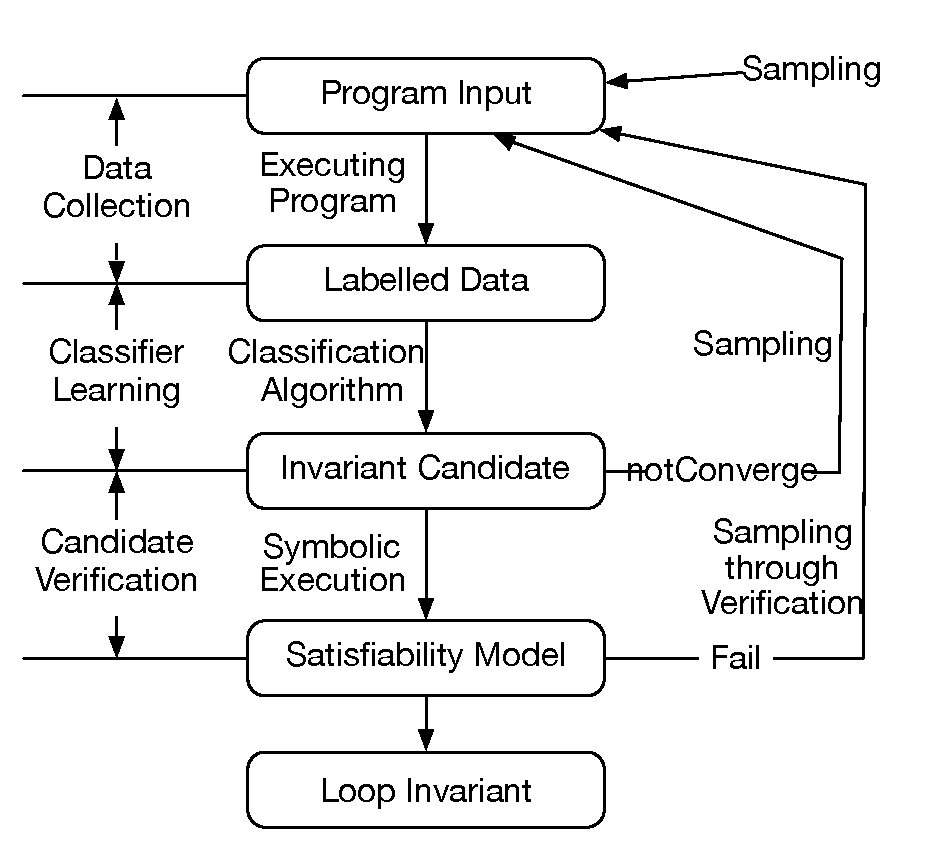
\includegraphics[scale=0.4]{figures/overview.pdf}
        \caption{Loop Invariant Inference Overview}
        \label{fig:overview}
    \end{minipage}%
    \begin{minipage}{.5\textwidth}
        \centering
        {\scriptsize\begin{verbatim}
        void func(int x, int y) {
            assume(x < y);
            while (x < y) {
                x = x + 100;
            }
            assert(x >= y && x < y + 99);
        }\end{verbatim}}
        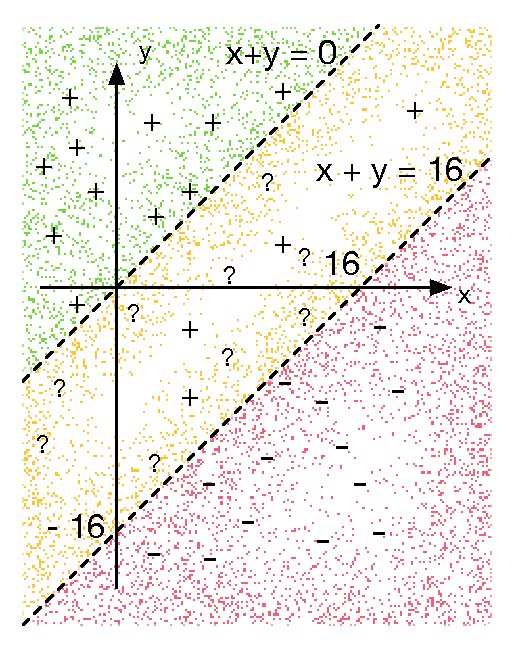
\includegraphics[scale=0.35]{figures/running-sampling.pdf}
        \caption{A Running Example}
        \label{example:running}
    \end{minipage}
\end{figure}

\medskip\noindent
\textbf{Overview.}
Our approach take the invariant reference as a refinement process 
based on iterations of data sampling, machine learning, concolic testing 
and constraint solving as shown in the Figure~\ref{fig:overview}. 
In the data sampling step, we execute the loop program $P$ based on three kinds of sampling sources: 
random sampling, selective sampling and counter-example sampling. 




